\thispagestyle{plain}
\chapter{Mathematical Optimization} \label{chap:optimization}
% \todo[inline]{brief introduction as in Huibert's thesis, shorten intro section, refer to book}
% \todo[inline]{link to other sections}
% Optimization appears in various disciplines. In timetabling, we seek a schedule at school such that teachers are assigned to students at a given time \cite{timetabling}. Of course different requirements have to be satisfied. Each teacher and student should have only one class at a time. The classes should not be too big and the teachers are only allowed to teach a limited number of hours per week. 
% Another example for an optimization problem is clustering, where we want to divide a set of data points into subsets that share similarities \cite{clustering}. 
% Optimization also arises in nature. Animals adapt and optimize their behaviour through learning \cite{optimization_systems_biology}.
% \todo[inline]{book Palsson, objective functions in practice; plus page 5 for evolution}
In mathematical optimization, the goal is to find an optimal solution that respects specific requirements. In particular, the behavior in cells can be modeled by mathematical optimization with biological objectives such as maximizing growth or minimizing energy usage \cite{intro_computational_systems_biology}. Optimization in cells is the topic of this thesis, and we will see in \cref{chap:metabolic_networks} how to use mathematical optimization to answer questions arising in systems biology. \\ 
In order to express a problem in practice mathematically, we need to formulate an objective and identify the constraints, i.e. the requirements in our system.
The resulting model is an \textit{optimization problem}, and we can use optimization algorithms to compute solutions. 
We define an optimization problem as:
\begin{mini!}
    {\scriptstyle \mathbf x \in \mathbb{R}^n}{f(\mathbf x)}{ \label[problem]{problem:optimization_problem}}{}
    \addConstraint{g_i(\mathbf x) \leq 0, \quad i=1,...,m} 
\end{mini!}

 where $f$ is the \textit{objective function}, $g_i$ are the \textit{constraint functions} and $\mathbf x$ are the \textit{decision variables}. %\cite{boyd_stephen_convex_2004}
The \textit{feasible region} is the set of points that respect the constraints. An optimization problem with a constrained feasible region is often also called \textit{constrained optimization problem} in contrast to an \textit{unconstrained optimization problem}. A \textit{solution} is a vector $\mathbf x$ that lies in the feasible region. An \textit{optimal solution} $\mathbf x^*$ is a solution with the smallest objective value. The \textit{objective value} of $\mathbf x^*$ is the value of the objective function evaluated at $\mathbf x^*$. If a problem has no solution, meaning that the constraints cannot be satisfied simultaneously, it is said to be \textit{infeasible}. A problem is \textit{unbounded} if solutions exist, but the objective value can be arbitrarily small. \vspace*{-\baselineskip}\newpage
One can maximize a function $f$ by setting the objective function to $\min -f(\mathbf x)$.\\
Depending on the type of objective function and the types of constraints, optimization problems are divided into different classes. The classes relevant for this thesis are linear programs, mixed-integer programs and disjunctive programs\footnote[1]{Program in this context does not mean a computer program. The term was coined in the 1950s and referred to planning in a military context. See \cite{understanding_lp} for more detail.}. 
Different algorithms can be used to solve optimization problems, which depend on the problem structure.
% \todo[inline]{or define solution as optimal solution}

\section{Linear Programming} \label{section:Linear Programming}
A \acfi{lp} is an optimization problem with a linear objective function and linear constraints.
\begin{mini!}
    {\scriptstyle \mathbf x}{\mathbf c^\intercal \mathbf x}{\label[problem]{problem:LP}}{}
    \addConstraint{\mathbf A \mathbf x\leq \mathbf b \quad \quad \quad} 
    \addConstraint{\mathbf x \in \mathbb{R}^n}
    % \addConstraint{x\geq \mathbf 0} 
\end{mini!}
 where $\mathbf c \in \mathbb{R}^n$, $ \mathbf A \in \mathbb{R}^{m \times n}$ and $\mathbf b \in \mathbb{R}^m$. It is assumed that the number of constraints $m$ is greater or equal to the number of variables $n$. %\unsure[inline]{to have an \textit{underdetermined} system of linear equations which allows to have many solutions} \todo[inline]{there can be many solutions regardless: e.g. a half space -> many solutions (M.)} 
We also assume that the columns of $\mathbf A$ are linearly independent.%\todo[inline]{ok?}
The linear inequalities define a polyhedron. If an optimal solution exists and if the feasible region has vertices%\todo[inline]{necessary?}
, there exists an optimal solution at one of the vertices. In that case, the LP can have exactly one optimal solution or multiple optimal solutions, for example, if an entire edge or face is optimal. An LP has no optimal solution if it is infeasible or unbounded.
\cref{problem:LP} is said to be in \textit{inequality form}%\unsure[inline]{ok to do so without constraints on x?} 
 ~\cite{boyd_stephen_convex_2004}.

As an example, we want to solve the following optimization problem: 
\begin{maxi!}
    {\scriptstyle x, y}{y}{ \label[problem]{problem:lp_example}}{}
    \addConstraint{0 \leq x \leq 3} 
    \addConstraint{0.5 \leq y \leq 4} 
    \addConstraint{y \leq 1.5 x + 0.5} 
    \addConstraint{y \leq -0.5 x + 4.5}
    \addConstraint{x,y \in \mathbb{R}}
\end{maxi!}
% \begin{equation} \label[problem]{problem:lp_example}
%     \text{max} \{y \, : \, 0 \leq x \leq 3 , \, 0.5 \leq y \leq 4, \, y \leq 1.5 x + 0.5, \, y \leq -0.5 x + 4.5, \, x,y \in \mathbb{R} \}
% \end{equation} 
The decision variables $x, y$ are continuous. We want to find a solution $(x^*, y^*)$ with maximal $y$-value such that the constraints are respected. The problem is a linear program and can be written as \cref{problem:LP} by simple linear transformations. If we want to write \cref{problem:lp_example} as a minimization problem, the objective becomes $-y$. If we visualize the example (\cref{fig:lp}), we see that there exists one optimal solution located at $(2,3.5)$. Usually, we are interested in problems in higher dimensions, and it is not possible to solve them visually.
% \todo[inline]{mention non-degeneracy?}
% \todo[inline]{why orthogonal line to objective function has the same objective values}

\begin{figure}[h!]
    \centering
    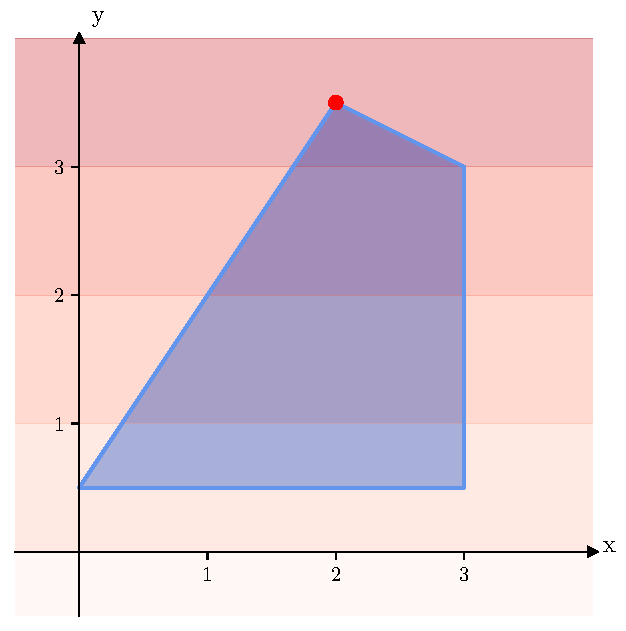
\includegraphics[width=0.5\textwidth]{Images/lp.pdf}
    \caption{\label{fig:lp} Visualization of LP (\cref{problem:lp_example})}
    \subcaption*{
        The set of feasible solutions contains all the points in the interior or on the boundary of the polytope (blue area). The optimal solution is the point in the feasible region with the biggest $y$-value (red point). The isolines indicate the function value of the points.}
\end{figure} 
% \unsure[inline]{remove grid?}

An LP is said to be in \textit{standard form} if it is of the form:
\begin{mini!}
    {\scriptstyle x}{\mathbf c^\intercal \mathbf x}{\label[problem]{problem:LP_standard_form}}{}
    \addConstraint{\mathbf A \mathbf x = \mathbf b} 
    \addConstraint{\mathbf x \geq \mathbf 0} 
\end{mini!}

 where $\mathbf c, \mathbf x \in \mathbb{R}^n, \, \mathbf A \in \mathbb{R}^{m \times n}$ and $\mathbf b \in \mathbb{R}^m$. 
\cref{problem:LP} can be written in standard form by adding one \textit{slack variable} per inequality to write it as equality \cite{noauthor_numerical_2006}. The constraint $\boldsymbol a_{i,*}^\intercal \mathbf x \leq b_i$ becomes $\boldsymbol a_{i,*} \,^\intercal \mathbf x + s_i = b_i$ with $s_i \geq 0$. Each variable $x_i$ that can be negative is replaced by $x_i^+ - x_i^-$, where $x_i^+ \geq 0$ and $x_i^- \geq 0$ \cite{noauthor_numerical_2006}.\\
A vertex of the feasible region is also called \textit{basic feasible solution}. Suppose we have an LP in standard form as in \cref{problem:LP_standard_form} with linearly independent rows. Let $\mathbf x \in \mathbb{R}^n$ be a basic feasible solution. There exist $m$ constraints that are a basis defining $\mathbf x$. $B$ is the set of constraint indices that are in the basis. Any variable $x_i \in B$ is a \textit{basic variable}. A variable $x_i \not \in B$ is a \textit{nonbasic variable} and $x_i=0$ \cite{understanding_lp}. 
% \todo[inline]{verify why constraint indices !!!}

\subsection{Solving LPs} \label{section:solving_lps}
There exist several algorithms to solve linear programs. The \textit{ellipsoid method} is the first algorithm that was proven to have a polynomial running time in the worst case. However, in practice, other algorithms outperform it \cite{understanding_lp}. 
Another class of algorithms is \textit{interior-point methods}. Some interior-point methods have a polynomial running time in the worst case and are often used in practice. Interior-point methods start with a feasible solution in the interior of the feasible region and approach the optimum without stepping outside the feasible region \cite{understanding_lp}. \\
Another algorithm that is relevant in practice is the \textit{simplex algorithm}. It is based on the fundamental property of LPs that the optimum is located at one of the vertices of the feasible region. %\todo[inline]{and that each vertex is corresponds to a basis, wrong words (M.)}. 
In \textit{phase \RomanNumeralCaps{1}} of the algorithm, a vertex of the feasible region is computed. In \textit{phase \RomanNumeralCaps{2}}, the algorithm moves from vertex to vertex along the edges of the feasible region until an optimum is found. The \textit{pivot rule} determines to which vertex the algorithm moves next. There exist several pivot rules, however, for all of them, there are families of problem instances on which the number of pivot steps needed grows exponentially. The worst-case running time on some instances conflicts with the observed polynomial running time in practice. Studying the simplex method with \textit{smoothed analysis}, which tries to close this gap, shows a polynomial running time of the simplex method. In smoothed analysis, a small noise is added to the entries of a fixed instance and afterward, worst-case analysis is performed on the perturbed instance \cite{huiberts,dadush}.
% \todo[inline]{when which algorithm is better}

\subsection{Optimality and Duality}
% \todo[inline]{transition}
To prove that a solution is optimal, we can use the \textit{Karush-Kuhn-Tucker}-conditions (KKT-conditions) and see the relation between the primal and the dual problems in LPs. 
An optimization problem can be written as an unconstrained problem by augmenting the objective function with a weighted sum of the constraints \cite{boyd_stephen_convex_2004}. The resulting function is known as the \textit{Lagrangian} function.
The Lagrangian of an LP in standard form is \cite{noauthor_numerical_2006}: 
\begin{equation} \label{Eq:lagrangian}
\mathcal{L} (\mathbf x, \boldsymbol{\lambda}, \boldsymbol \nu) = \mathbf c^\intercal \mathbf x - \sum_{i=1}^n \lambda_i x_i - \sum_{i=1}^m \mathbf \nu_i (A_{i,*}^\intercal \mathbf x - b_i)
\end{equation} %\todo[inline]{$\lambda_i (x_i)$ correct?}
 where $\lambda_i \geq 0$ and $\nu_i \in \mathbb{R}$ are called \textit{Lagrange multipliers} or \textit{dual variables}.
As the objective function of linear programs is convex, the KKT-conditions are a proof for global optimality of a solution. We obtain the optimality conditions captured in \cref{theorem:lp_duality}. 

\begin{theorem}[Optimality conditions for LPs] \label{theorem:lp_duality}
    A solution $\mathbf x^*$ is optimal if there exist vectors $\boldsymbol \lambda$ and $\boldsymbol \nu$ that satisfy the following conditions \cite{noauthor_numerical_2006}:
    \begin{enumerate}
        \item $\boldsymbol \lambda + \mathbf A^\intercal \boldsymbol \nu = \mathbf c $ \hfill (stationarity)
        \item $ \mathbf A \mathbf x - \mathbf b = \mathbf 0$ \hfill (primal feasibility)
        \item $\mathbf x \geq \mathbf 0$ \hfill (primal feasibility)
        \item $\boldsymbol \lambda \geq \mathbf 0$ \hfill (dual feasibility)
        \item $\mathbf x^\intercal \boldsymbol \lambda = \mathbf 0$ \hfill (complementary slackness)
    \end{enumerate}
\end{theorem} 
We call a linear program in standard form as in \cref{problem:LP_standard_form} the \textit{primal problem}~($\mathcal{P}$).
The associated \textit{dual function} of the primal problem is \cite{aps_mosek_nodate, boyd_stephen_convex_2004}:
%\todo[inline]{MB: shouldn't the conditions $x \geq 0, \lambda \geq 0$ appear somewhere?}
\begin{align*}
    q(\boldsymbol \lambda, \boldsymbol \nu)
    & = \inf_{\mathbf x} \mathcal{L} (\mathbf x, \boldsymbol \lambda, \boldsymbol \nu) \\
    & = \inf_{\mathbf x} \mathbf c^\intercal \mathbf x - \boldsymbol \lambda^\intercal \mathbf x - \boldsymbol \nu^\intercal (\mathbf A \mathbf x - \mathbf b) & \\
    & = \inf_{\mathbf x} \mathbf c^\intercal \mathbf x - \boldsymbol \lambda^\intercal \mathbf x - \boldsymbol \nu^\intercal \mathbf A \mathbf x + \boldsymbol \nu^\intercal \mathbf b  &\\
    & = \inf_{\mathbf x} (\mathbf c^\intercal - \boldsymbol \lambda^\intercal - \boldsymbol \nu^\intercal \mathbf A) \mathbf x + \boldsymbol \nu^\intercal \mathbf b  &\\
    & = \inf_{\mathbf x} \mathbf x^\intercal (\mathbf c - \boldsymbol \lambda - \mathbf A^\intercal \boldsymbol \nu) + \mathbf b^\intercal \boldsymbol \nu &\\
    & = \left\{
    \begin{array}{lr}
        \mathbf b^\intercal \boldsymbol \nu \quad \quad \text{if} \, \, \mathbf c - \boldsymbol \lambda - \mathbf A^\intercal \boldsymbol \nu = \mathbf 0\\
        - \infty \quad \quad \text{otherwise}
    \end{array}
    \right.
\end{align*}

% \todo[inline]{check if it has to be inf}
Let $\mathbf x^P$ be a feasible solution to the primal problem, and let $(\boldsymbol \lambda^D, \, \boldsymbol \nu^D)$ be a feasible solution to the dual problem. If the dual function is bounded we know that $\mathbf c - \boldsymbol \lambda^D = \mathbf A^\intercal \boldsymbol \nu^D$ and we know that $\mathbf x^P$ satisfies $ \mathbf A\mathbf x^P = \mathbf b$. The function value $q(\boldsymbol \lambda^D, \boldsymbol \nu^D)$ is a lower bound on the objective value of the primal problem \cite{aps_mosek_nodate}: 
\begin{equation*}
    \mathbf b^\intercal \boldsymbol \nu^D
    = (\mathbf A \mathbf x^P)^\intercal \boldsymbol \nu^D 
    = \mathbf {x^P}^\intercal \mathbf A^\intercal \boldsymbol \nu^D 
    = \mathbf {x^P}^\intercal (\mathbf c - \boldsymbol \lambda^D) 
    = \mathbf c^\intercal \mathbf x^P  - \boldsymbol {\lambda^D}^\intercal \mathbf x^P
    \leq \mathbf c^\intercal \mathbf x^P
\end{equation*}
The tightest bound maximizes $\mathbf b^\intercal \boldsymbol \nu$. Formulated as a linear program we obtain the \textit{dual problem} ($\mathcal{D}$):
\begin{maxi!}
    {\scriptstyle \boldsymbol \nu, \boldsymbol \lambda}{\mathbf b^\intercal \boldsymbol \nu}{\label[problem]{problem:dual_problem_slack}}{}
    \addConstraint{\boldsymbol \lambda + \mathbf A^\intercal \boldsymbol \nu = \mathbf c} 
    \addConstraint{\boldsymbol \lambda \geq \mathbf 0} 
\end{maxi!}
or rewritten without the slack variables $\boldsymbol \lambda$ \cite{noauthor_numerical_2006}:
\begin{maxi!}
    {\scriptstyle \boldsymbol \nu}{\mathbf b^\intercal \boldsymbol \nu}{\label[problem]{problem:dual_problem}}{}
    \addConstraint{\boldsymbol A^\intercal \boldsymbol \nu \leq \mathbf c} 
\end{maxi!}
% \unsure[inline]{add dimensions to all variables}
Let $p^*$ be the objective value of an optimal solution to the primal problem and $d^*$ the objective value of an optimal solution to the dual problem. We have seen that $d^*$ is a lower bound on $p^*$ which is known as \textit{weak duality}. We speak of \textit{strong duality} if $p^*=d^*$. 

\begin{theorem}[Strong Duality] \label{theorem:strong_duality}
    Given a primal $\mathcal{P}$ and corresponding dual \\program~$\mathcal{D}$, exactly one of the following is true \cite{noauthor_numerical_2006}:
    \begin{enumerate}
        \item $\mathcal{P}$ and $\mathcal{D}$ both have at least one optimal solution. If $p^*$ is the objective value of an optimal solution to $\mathcal{P}$ and $d^*$ is the objective value of an optimal solution to $\mathcal{D}$, then $p^*=d^*$.
        \item Either $\mathcal{P}$ or $\mathcal{D}$ is unbounded and the other is infeasible. 
        \item $\mathcal{P}$ and $\mathcal{D}$ both are infeasible.
    \end{enumerate}
\end{theorem}
% For linear programs, \textit{strong duality} holds. 
A proof for \cref{theorem:strong_duality} can be found in \cite{aps_mosek_nodate}. Property (1) of \cref{theorem:strong_duality} can be used to prove the optimality of a solution. 

We have seen how to derive the dual problem of an LP in standard form. We do not require an LP in standard form to derive the corresponding dual problem. For example, the dual problem of \cref{problem:LP} is: 
\begin{maxi!}
    {\scriptstyle \boldsymbol \mu}{\mathbf b^\intercal \boldsymbol{\mu}}{\label[problem]{problem:LP_dual}}{}
    \addConstraint{\mathbf A^\intercal \boldsymbol{\mu} = \mathbf c} 
    \addConstraint{\mu_i \geq 0}
    % \addConstraint{x\geq \mathbf 0} 
\end{maxi!}

% \todo[inline]{example + visualization}
% \begin{lemma}[Farkas Lemma]
%     Given an LP in standard form, exactly one of the following is true:
%     \begin{enumerate}
%         \item the LP has at least one solution $x$
%         \item there exists a vector $y$ such that $ \mathbf A^\intercal y \leq 0$ and $b^\intercal y > 0$
%     \end{enumerate}
% \end{lemma}

% \cite{aps_mosek_nodate}

\newpage
\section{Mixed-Integer Programming} \label{section:MIP}
Many problems in practice cannot be formulated by only using linear constraints and continuous decision variables. It is often required that a subset of variables is discrete. A \acfi{mip} is an optimization problem with a linear objective function, linear constraints and a subset of integer variables:
\begin{mini!}
    {\scriptstyle \mathbf x}{\mathbf c^\intercal \mathbf x}{\label[problem]{problem:MIP}}{}
    \addConstraint{\mathbf A \mathbf x\leq \mathbf b} \label[constraint]{constraint:MIP_inequality}
    % \addConstraint{x\geq \mathbf 0} 
    \addConstraint{\mathbf x \in \mathbb{Z}^{|J|} \times \mathbb{R}^{n-|J|} \label[constraint]{constraint:MIP_integer}
    }
\end{mini!}
 where $\mathbf c \in \mathbb{R}^n, \, \mathbf A \in \mathbb{R}^{m \times n}$, $\mathbf b \in \mathbb{R}^m$. The set $J$ contains the indices of integer variables. 

Let us reuse the LP example in \cref{section:Linear Programming} and add integrality constraints on the decision variables $x$ and $y$:
\begin{maxi!}
    {\scriptstyle x, y}{y}{ \label[problem]{problem:mip_example}}{}
    \addConstraint{0 \leq x \leq 3} 
    \addConstraint{0.5 \leq y \leq 4} 
    \addConstraint{y \leq 1.5 x + 0.5} 
    \addConstraint{y \leq -0.5 x + 4.5}
    \addConstraint{x,y \in \mathbb{Z}}
\end{maxi!}
% \begin{equation} \label[problem]{problem:mip_example}
%     \text{max} \{y \, : \, 0 \leq x \leq 3 , \, 0.5 \leq y \leq 4, \, y \leq 1.5 x + 0.5, \, y \leq -0.5 x + 4.5, \, x,y \in \mathbb{Z} \}
% \end{equation} 
Looking at the visualization of the problem (\cref{fig:mip}), we see that the optimal solution of the LP $x^{LP} = (2,3.5)$ is no valid solution to the MIP formulation. The points $(2,3)$ and $(3,3)$ are the optimal solutions.

\begin{figure}[h!]
    \centering
    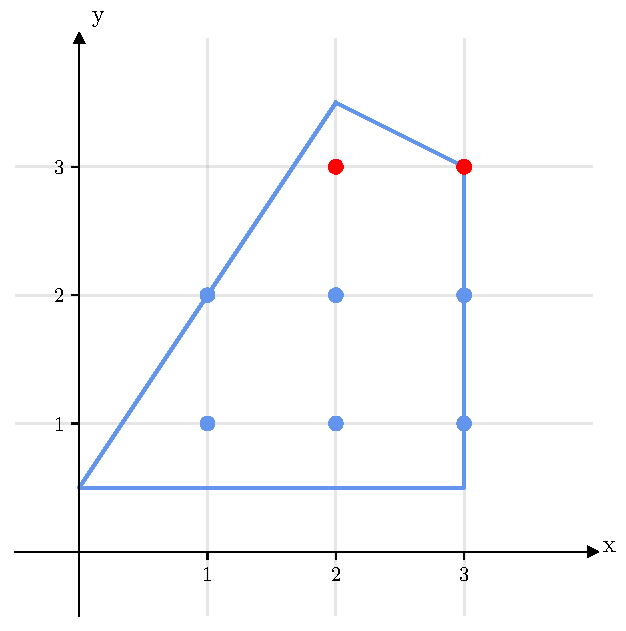
\includegraphics[width=0.5\textwidth]{Images/mip.pdf}
    \caption{Visualization of MIP (\cref{problem:mip_example})}
    \label{fig:mip}
    \subcaption*{
        The feasible points of the MIP are the integer points respecting the polyhedral constraints (blue points). The set of feasible solutions to the relaxed LP are all the points in the interior or on the boundary of the polytope (blue line segments). An optimal solution is a point in the feasible region with the biggest $y$-value (red point). The optimal solutions are at $(2,3)$ and $(3,3)$.}
\end{figure}

The MIP formulation enables us to model much more complex problems. Apart from incorporating discrete quantities, it is possible to capture Boolean expressions. Suppose we want to model the \textit{indicator constraint} $z = 1 \implies \boldsymbol a^\intercal \mathbf x \leq b$. We can reformulate the constraint with a linear constraint using the \textit{big-M method}: 
\begin{equation*}
    \boldsymbol a^\intercal \mathbf x \leq b + M(1-z)
\end{equation*}
If $z=1$ the constraint is enforced. In the case $z=0$, the value of $M$ has to be larger than $\boldsymbol a^\intercal \mathbf x - b$ for any $\mathbf x$ such that the constraint is inactive \cite{aps_mosek_nodate}.

\subsection*{Solving MIPs} %\addcontentsline{toc}{subsubsection}{\protect\numberline{}Solving MIPs}
Solving MIPs is much more complicated than solving LPs, because it is not guaranteed that if an optimal solution exists, it is at one of the vertices. 
In general, solving MIPs is $\mathcal{NP}$-hard. A problem is in $\mathcal{NP}$ if a solution is verifiable in polynomial time. A problem is $\mathcal{NP}$-hard if it requires at least as much time to solve the problem as any other problem that is in $\mathcal{NP}$. $\mathcal{NP}$-complete problems are $\mathcal{NP}$-hard and are in $\mathcal{NP}$ \cite{CormenIntroduction}. 
In complexity theory, problems are usually defined as decision problems. 
The decision problem of \cref{problem:MIP} would be "Is the feasible region nonempty?", which is $\mathcal{NP}$-complete \cite{integer_programming}. 
As finding an optimal solution is not easier than finding any solution, it follows that MIPs are $\mathcal{NP}$-hard \cite{integer_programming}.
% NP: set of decision problems solvable in polynomial time and verifiable in polynomial time 
% NP-hard: polynomial time reduction from an NP-complete problem G to H -> H can be optimization problem
% 0-1 integer linear programmings is NP-complete
% MILP feasibility problem is in NP:
% - yes verifiable in polynomial time
% - 
% \todo[inline]{verify correctness, add reduction}
% Achtung! NP-hard problems müssen nicht zwangsweise Decision Problems sein, NP und NP-complete problems aber schon!
% Inbesondere muss sich ein NP-hard problem auf ein NP-completes problem (in poly zeit) reduzieren lassen, ergo wenn ich einen polynomischen Lösungansatz für das zweite habe, habe ich auch einen für das erste.

Instead of solving the MIP directly, one can solve a sequence of \textit{LP relaxations}: the integrality constraints are ignored and \cref{constraint:MIP_integer} becomes $\mathbf x \in \mathbb{R}^n$.
Let $z^{LP}$ be the objective value of an optimal solution $\bold{x}^{LP}$ of the LP relaxation and $z^*$ the objective value of an optimal solution $\bold{x^*}$ to the MIP problem.\\
We know that: 
\begin{equation*} \label{Eq:bound}
    z^{LP} \leq z^*
\end{equation*}
\newpage
One common approach for solving MIPs is the \textit{branch-and-bound} algorithm \cite{integer_programming}. The idea is to generate a branch-and-bound tree starting with the solution to the LP relaxation $\mathbf x^{LP} \in \mathbb{R}^n$ at the root node. A variable $x_i$ that is fractional in $\mathbf x^{LP}$ and violates the integrality constraint is selected as \textit{branching variable}. We divide the search space $P$ by creating two child nodes. In one $x_i$ has to be larger or equal to the ceiled value and the feasible region becomes $P \cap \{x_i \geq \lceil x_i^{LP} \rceil \}$. In the other child node, $x_i$ can take at most the floored value of $x_i^{LP}$ and the feasible region of the subproblem is $P \cap \{x_i \leq \lfloor x_i^{LP} \rfloor \}$. The solution with the smallest objective value respecting the MIP formulation is called \textit{incumbent} and the objective value is denoted by $z^{INC}$. We continue branching until all variables in $J$ are integral, a subproblem is infeasible or a node can be $pruned$. The optimal solution in each node $i$ is bounded by the objective value of the relaxed solution $z^{LP}_{(i)}$. If $z^{LP}_{(i)}$ is greater or equal to $z^{INC}$, node $i$ is cut off the tree. \\
Another approach to solve MIPs is the \textit{cutting plane} algorithm \cite{integer_programming}. The LP relaxation can be very weak. As we are dealing with a linear objective, we could get the optimal MIP solution easily if we had access to the \textit{integer hull}: $\text{conv}(P \cap \mathbb{Z}^n)$. If the LP relaxation does not correspond to the integer hull, one can tighten the LP relaxation by adding \textit{cuts}. A cut is an inequality that does not cut off any feasible solution (see \cref{section:cuts}). Given a relaxed solution $\mathbf x^{LP}$ that violates at least one integer constraint, one separates $\mathbf x^{LP}$ from the hull with a cut. This process is repeated until $\mathbf x^{LP}$ is an optimal solution to the MIP. \\
A combination of the branch-and-bound algorithm and the cutting plane algorithm is the \textit{branch-and-cut} algorithm \cite{integer_programming}. The LP relaxation at a node is potentially tightened by adding cuts. 

\newpage
\section{Disjunctive Programming}
% \todo[inline]{motivation from MIP to DP}
Often, the requirements of a problem are complex, and linear constraints are not sufficient for modeling. With Boolean expressions, more complicated relationships between variables can be captured. % without using the big-M formulation.     
A \acfi{dp} is an optimization problem with linear constraints, continuous variables and logical constraints:
\begin{mini!}
    {\scriptstyle \mathbf x}{\mathbf c^\intercal \mathbf x}{\label[problem]{problem:DP}}{}
    \addConstraint{\mathbf A \mathbf x\leq \mathbf b} 
    \addConstraint{\bigvee_{i \in Q_j} \{\mathbf d^{(i)\intercal} \mathbf x \leq d_{0}^i\} \quad \forall j \in S} 
\end{mini!}
 where $\mathbf c, \mathbf x \in \mathbb{R}^n$, $ \mathbf A \in \mathbb{R}^{m \times n}$, $\mathbf b \in \mathbb{R}^m$, $\mathbf d^{(i)} \in \mathbb{R}^n$ and $d_{0}^i \in \mathbb{R}$. The set $S$ is the set of disjunction indices.
As the terms $i$ in each disjunction $Q_j$ are linear, each disjunctive set is a polyhedron. The feasible region is in general non-convex due to the disjunctive constraints \cite{balas_disjunctive_2018}. 
Alternatively, the disjunctions can be captured by Boolean variables $Y_{ij} \in \{true, false \}$, where $Y_{ij}$ corresponds to the $i$-th disjunct in disjunction $j$:
\begin{mini!}
    {\scriptstyle \mathbf x}{\mathbf c^\intercal \mathbf x}{\label[problem]{problem:DP_bool}}{}
    \addConstraint{\mathbf A \mathbf x\leq \mathbf b} 
    \addConstraint{\bigvee_{i \in Q_j} \left[ \begin{array}{c}  
        Y_{ij}\\ 
        \{\mathbf d^{(i)\intercal} \mathbf x \leq d_{0}^i\}
    \end{array} \right] \quad \forall j \in S \quad \quad \quad \quad} 
    \addConstraint{\Omega (Y) = true}
\end{mini!}

As an example, we want to solve the following optimization problem:
% \begin{align} 
%     \begin{split}
%     \text{max} \{y \, : \, &((0 \leq x \leq 1) \land (0.5 \leq y \leq 1.5 x + 0.5)) \, \lor \\ &((2 \leq x \leq 3) \land (0.5 \leq y \leq -0.5 x + 4.5))  \, x,y \in \mathbb{R} \}
%     \end{split}
% \end{align} 
\begin{maxi!}
    {\scriptstyle x, y}{y}{\label[problem]{problem:dp_example}}{}
    \addConstraint{\begin{aligned}\bigl((0 \leq x \leq 1) \land (0.5 \leq y \leq 1.5 x + 0.5)\bigr) \, \, \lor \\ \bigl((2 \leq x \leq 3) \land (2 \leq y \leq -0.5 x + 4.5)\bigr) \end{aligned}} 
    \addConstraint{x,y \in \mathbb{R}} 
\end{maxi!}

The feasible region is the union of two polyhedra and no longer convex. The optimal solution is the point with maximal value in either of the polytopes and located at $(2, 3.5)$ which we see in the visualization (\cref{fig:dp}). 

\begin{figure}[h!]
    \centering
    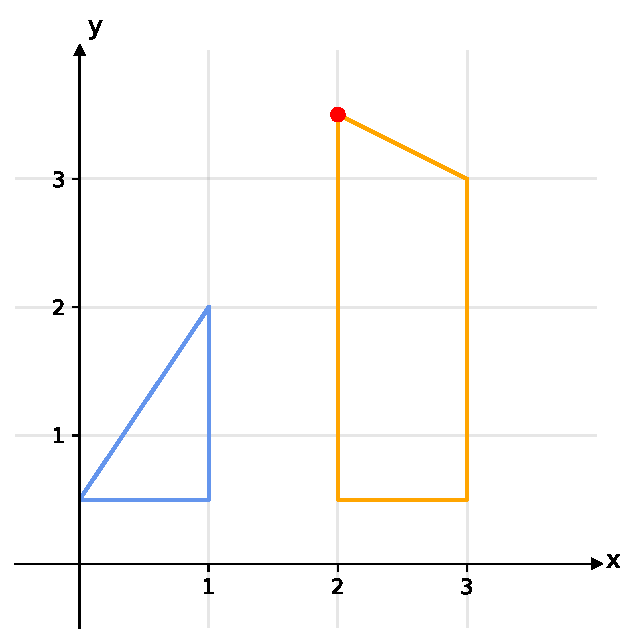
\includegraphics[width=0.5\textwidth]{Images/dp.pdf}
    \caption{Visualization of DP (\cref{problem:dp_example})}
    \label{fig:dp}
    \subcaption*{
        The set of feasible solutions is no longer convex and is the union of the polytope $P_1$ (blue area) and the polytope $P_2$ (orange area). The optimal solution is the point in the feasible region with the biggest $y$-value (red point).}
\end{figure}
% \unsure[inline]{write problem in dp form?}

\subsection*{Solving DPs} %\addcontentsline{toc}{subsubsection}{\protect\numberline{}Solving DPs} 
\label{section:solving_dps}
% \todo[inline]{mention big-M only in half sentence, DPs offer a different type of constraint, align with intro to DPs}
A disjunctive model can be formulated as a mixed-integer program and solved by corresponding techniques (see \cref{section:MIP}). Disjunctions can be expressed by linear constraints and integer variables by using the big-M method. \\
% Suppose we have a disjunction with $k$ terms:
% \begin{equation*}
%     (\boldsymbol a_1^\intercal \mathbf x \leq b_1) \lor (\boldsymbol a_2^\intercal \mathbf x \leq b_2) ... \lor (\boldsymbol a_k^\intercal \mathbf x \leq b_k)
% \end{equation*}
% We use the binary variable $y_i$ and enforce with the constraint $y_1 +  y_2 + ... + y_k \geq 1$ that at least one of the $k$ terms is true. If $y_i=1$, term $(\boldsymbol a_i^\intercal \mathbf x \leq b_i)$ is enforced. See \cref{section:MIP} on how to express indicator constraints with linear constraints and binary variables. Often, the $M$ constant has to be large to be inactive if $y_i=0$. However, a large $M$ leads to a weaker LP relaxation which impacts the running time of the Branch-and-Bound algorithm \cite{aps_mosek_nodate}. 
Another possibility is to convexify the feasible region and solve the resulting linear program. The idea is to build the convex hull of the union of polyhedral points in a higher dimension. The optimal solution at a vertex of the convex hull is optimal for the disjunctive program, as we are dealing with linear constraints. % and project the solution back to the original dimension of the problem. 
For an example of how to write a disjunctive program using the big-M or the hull reformulation, we refer to \cite{perez_disjunctiveprogrammingjl_2023}.
\cref{fig:dp_solving_techniques} shows the 2D projection of the big-M reformulation and the convex-hull formulation of a disjunctive program. \newpage

\vspace*{0.5cm}
% \unsure[inline]{how to solve if corner can be infeasible?}
\begin{figure}[H]
    \centering
    \caption{DP reformulations}
    \label{fig:dp_solving_techniques}
    \begin{subfigure}{0.33\textwidth}
    \centering
        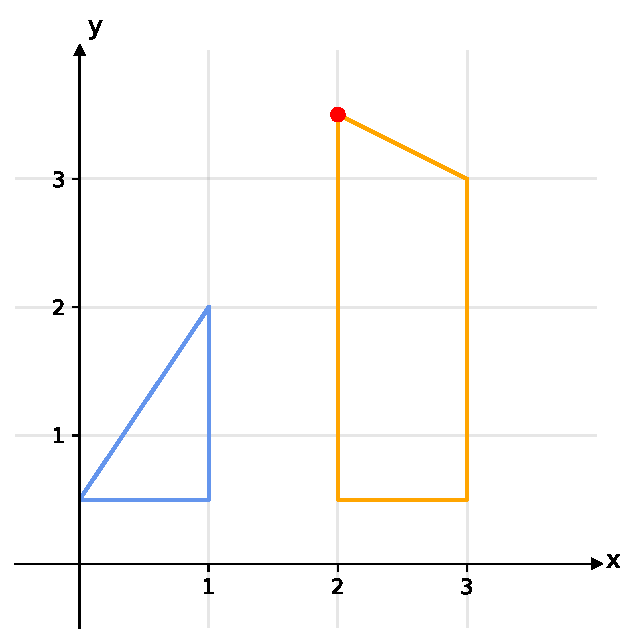
\includegraphics[width=0.95\linewidth]{Images/dp.pdf}
        \caption{}
    \end{subfigure}%
    \begin{subfigure}{0.33\textwidth}
    \centering
        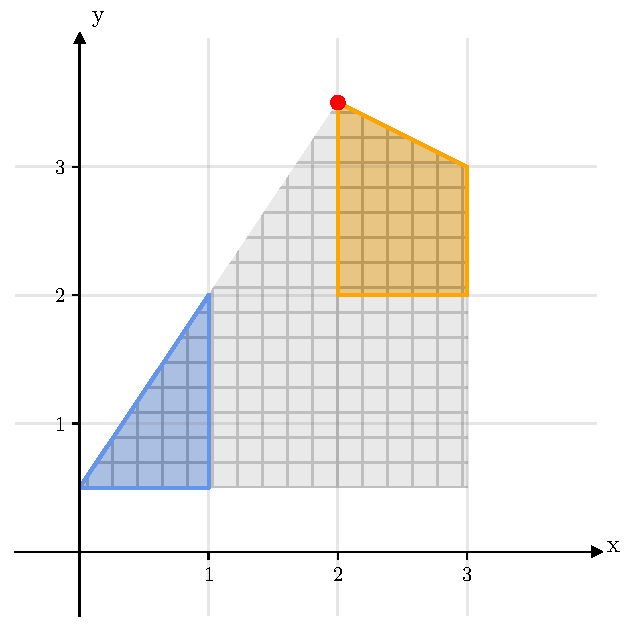
\includegraphics[width=0.95\linewidth]{Images/dp_big_m.pdf}
        \caption{}
    \end{subfigure}
    \begin{subfigure}{0.33\textwidth}
    \centering
        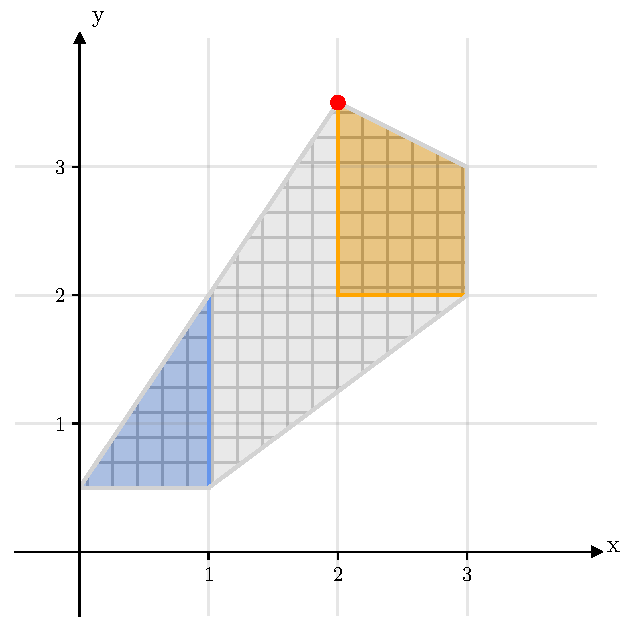
\includegraphics[width=0.95\linewidth]{Images/dp_convex_hull.pdf}
        \caption{}
    \end{subfigure}
    \subcaption*{The feasible region of a disjunctive program (a), the approximation of the region using the big-M reformulation (b) and the convex-hull formulation (c). The plot is inspired by \cite{hutchison_automating_2010}.}
\end{figure}

\section{Decompositions and Cutting Planes} \label{section:cuts}
Let us consider a mixed-integer problem (\cref{problem:MIP}) with decision variables $\mathbf x$. A \textit{cutting plane} or \textit{cut}, parameterized by $\boldsymbol \alpha \in \mathbb{R}^{n+1}$, is an inequality that when added to the MIP does not remove any feasible solution and is defined as: 
\begin{equation} \label{Eq:cuts}
    \sum_{i=1}^n \alpha_i x_i \leq \alpha_0 \quad  \forall \mathbf x \in P \cap S
\end{equation} 
 where $\alpha_i \in \mathbb{R}$, $P$ is the polyhedron defined by the inequality in \cref{constraint:MIP_inequality}, and $S$ is the set of points satisfying \cref{constraint:MIP_integer}. Usually, cutting planes are used to cut off solutions to the relaxed problem that are infeasible in the original problem. 

\cref{fig:cuts} shows a visualization of \cref{problem:mip_example} in which the relaxed solution $\mathbf x^{LP}$ is not feasible in the MIP. The relaxed solution $\mathbf x^{LP}$ is separated from the integer hull by cuts.

\begin{figure}[!h]
    \centering
    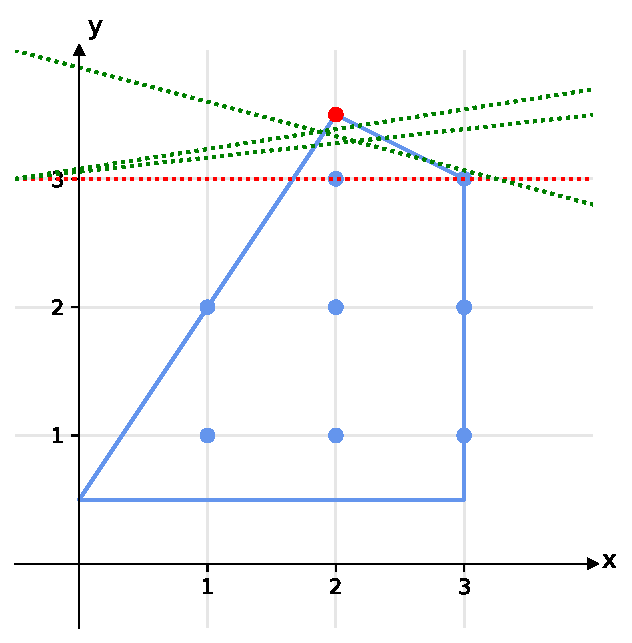
\includegraphics[width=0.5\textwidth]{Images/mip_cut.pdf}
    \caption{Tightening a relaxed problem with cuts (\cref{problem:mip_example})}
    \label{fig:cuts}
    \subcaption*{The feasible points of \cref{problem:mip_example} are the integer points within the polytope. In the relaxed problem, the integrality constraints are ignored. The relaxed solution is $\mathbf x^{LP}=(2, 3.5)$. As $\mathbf x^{LP}$ is not an integer solution, it is cut off by adding cuts. The tightest cut is indicated by the red dashed line.}
\end{figure}
% \unsure[inline]{update caption, the relaxed problem is fix}

For a relaxed solution $\mathbf x^{LP}$ with $\mathbf x^{LP} \notin P \cap S$, there exist multiple hyperplanes separating $\mathbf x^{LP}$ from the actual feasible region. %\todo[inline]{MB: if you think of it, can there exists conditions where a unique hyperplane would separate a point from a convex set?}
As we want to tighten the search space, we are interested in cuts that cut off many infeasible points at once. There are different scores to estimate the quality of a cut \cite{turner_adaptive_2023}.
\newpage
One scoring measure is \textit{efficacy} which is the signed distance from $\mathbf x^{LP}$ to the cutting plane:
\begin{equation}
    \text{eff}(\boldsymbol \alpha, \mathbf x^{LP}) := \frac{\boldsymbol \alpha^\intercal \mathbf x^{LP} - \alpha_0}{\lVert \boldsymbol \alpha \rVert}
\end{equation}

However, there is a tradeoff between the quality of a cut and the complexity of generating it.
% \todo[inline]{differentiate between cut and decomposition}
% The cuts relevant for this thesis are explained in detail below. 
% \todo[inline]{numerical issues}

\todo[inline]{decomposition if variables of original problem are projected out; cut if we have a valid inequality \\
Decomposition for no-good cuts and combinatorial Benders'\\
intersection cuts are actual cuts}

\subsection{Decomposition with No-Good Cuts}
Given an integer problem P as in \cref{problem:MIP} with only binary variables: $|J|=n$ and $x_i \in \{0,1\}$. 
We can decompose P into a relaxed problem and solve a subproblem to check whether a relaxed solution lies in the feasible region of the original problem. If a relaxed solution is not feasible in the original problem, we add a cut to the relaxed problem to remove the relaxed solution from the search space. \\
Let $\mathbf x^{IP}$ a solution to the relaxed integer program, where \cref{constraint:MIP_inequality} is relaxed. We further assume that $\mathbf x^{IP}$ is not a feasible solution to P. The following \textit{no-good cut} is added to the relaxed IP and forbids the assignment of integer variables in $\mathbf x^{IP}$:
\begin{equation*}
    \sum_{j \in J: x_j^{IP}=0} (1 - x_{j}) + \sum_{j \in J: x_j^{IP}=1} x_j \quad \leq \quad |J| -1
\end{equation*}
Such a cut usually tightens the feasible region of P marginally and it would require a large number of no-good cuts to arrive at the integer hull.

\subsection{Combinatorial Benders' Decomposition} \label{section:optimization_CB}
Instead of forbidding one assignment of variables as with a no-good cut, with combinatorial Benders' cuts, we generate stronger cuts, by identifying the subset of variables that lead to the infeasibility. This section is based on \cite{codato_combinatorial_2006}.

Given a problem of the form:
\begin{mini!}
    {\scriptstyle \mathbf x, \mathbf z}{\mathbf c^\intercal \mathbf x}{\label[problem]{problem:mathematical_program_CB}}{} 
    \addConstraint{\mathbf F \mathbf x \leq \mathbf g}
    \addConstraint{\mathbf D \mathbf z \leq \mathbf e}
    \addConstraint{x_j = 1 \implies \boldsymbol a_{i,*}^\intercal \mathbf z \leq b_i \quad \forall i \in I} \label[constraint]{constraint:mathematical_program_CB_d}
    \addConstraint{x \in \{ 0,1 \}^n}
    \addConstraint{z_i \in \mathbb{R}}
\end{mini!} 
As the objective does not depend on $\mathbf z$ and as the decision variables $\mathbf x, \mathbf z$ are independent apart from the indicator constraints, we can split the problem into a \acfi{mp} and a \acfi{sp}. \cref{constraint:mathematical_program_CB_d} can be reformulated using the big-M method: $\mathbf A \mathbf z \leq \mathbf b + M(\mathbf 1- \mathbf x)$. 

In the master problem, the constraints on $\mathbf z$ are ignored: 
\begin{mini!}
    {\scriptstyle \mathbf x}{\mathbf c^\intercal \mathbf x}{\label[problem]{problem:MP}}{}
    \addConstraint{\mathbf F \mathbf x \leq \mathbf g}    
    \addConstraint{\mathbf x \in \mathbb{R}^n}
    \addConstraint{x_j \in \{ 0,1 \}}
\end{mini!}

The subproblem depends on a solution $\mathbf x^{MP}$ to the master problem. 
\begin{mini!}
    {\scriptstyle \mathbf z}{0}{\label[problem]{problem:SP}}{}
    \addConstraint{\mathbf D \mathbf z \leq \mathbf e}
    \addConstraint{\boldsymbol a_{i,*}^\intercal \mathbf z \leq b_i + M(1- x_{j}^{MP}) \quad \forall i \in I \quad}
\end{mini!}
% \unsure[inline]{write M as matrix, vector or constant}
\newpage
If solution $\mathbf x^{MP}$ leads to a feasible subproblem, $\mathbf x^{MP}$ is an optimal solution to \cref{problem:mathematical_program_CB}. If the problem is infeasible, $\mathbf x^{MP}$ is not a feasible solution to the original problem in which case we want to add a cut that removes $\mathbf x^{MP}$ from the search space. Suppose we have access to a \acfi{mis} $C$ that is an inclusion-wise minimal set of row indices corresponding to the constraints in the subproblem that lead to infeasibility.\\
The subproblem can then be written as:
\begin{mini!}
    {\scriptstyle \mathbf z}{0}{}{}
    \addConstraint{\mathbf D \mathbf z \leq \mathbf e}
    \addConstraint{\boldsymbol a_{i,*}^\intercal \mathbf z \leq b_i + M_i(1- x_{j}^{MP}) \quad \forall i \in C}
\end{mini!}
% \todo[inline]{MB: do you even need big M constraints in the expression? The point of CB is precisely to avoid big M \\-> taken from \cite{codato_combinatorial_2006}}
The \textit{combinatorial Benders' cut} is then: 
\begin{equation*}
    \sum_{j \in C: x_j^{MP}=0} (1 - x_{j}) + \sum_{j \in C: x_j^{MP}=1} x_j \quad \leq \quad |C| -1
\end{equation*}

A minimal infeasible subsystem can be found by studying the dual problem of the infeasible subproblem. As the subproblem is a linear problem, strong duality holds and an infeasible primal problem implies an unbounded dual problem (see \cref{section:Linear Programming}).

To derive the dual problem of \cref{problem:SP} we write constraints (b) and (c) as one constraint and stack the variables in the vector $\mathbf y$: $\bold{\tilde A} \mathbf y \leq \bold{\tilde b}$. \\
The dual is then:
\begin{maxi!}
    {\scriptstyle \boldsymbol \lambda}{\bold{\tilde b}^\intercal \boldsymbol \lambda}{\label[problem]{problem:primal_cb}}{}
    \addConstraint{\bold{\tilde A}^\intercal \boldsymbol \lambda = \mathbf 0}
    \addConstraint{\boldsymbol \lambda \geq \mathbf 0}
\end{maxi!}

As $\boldsymbol \lambda = \bold 0$ is a feasible solution to the dual problem, the dual problem is unbounded, and there exist multiple feasible solutions. We are interested in a feasible solution with $\boldsymbol \lambda \neq \mathbf 0$ and therefore add the constraint $\bold{\tilde b}^\intercal \boldsymbol \lambda = \mathbf 1$. Now that the objective function is hidden in the constraints, we can set a different objective function. 

The linear program to find minimal infeasible subsystems is then:
\begin{maxi!}
    {\scriptstyle \boldsymbol \lambda}{\sum_i w_i \lambda_i}{\label[problem]{problem:mis_lp}}{} 
    \addConstraint{\bold{\tilde A}^\intercal \boldsymbol \lambda = \mathbf 0}
    \addConstraint{\boldsymbol \lambda \geq \mathbf 0}
    \addConstraint{\bold{\tilde b}^\intercal \boldsymbol \lambda = \mathbf 1}
\end{maxi!}
 where $w_i$ is the weight corresponding to the dual variable $\lambda_i$. The support of each solution at a vertex of the feasible region of \cref{problem:mis_lp}  defines a minimal infeasible subsystem. By changing the weights in the objective, several MISs can be obtained for one infeasible MP solution. 


\subsection{Intersection Cuts} \label{section:optimization_intersection_cuts}

Suppose we are given a problem of the form:
\begin{mini!}
    {\scriptstyle \mathbf x}{\mathbf c^\intercal \mathbf x}{}{} \label[problem]{problem:mathematical_program_S_P}
    \addConstraint{\mathbf x \in S \cap P}
\end{mini!} 
 where $\mathbf c \in \mathbb{R}^n$, $P$ is a polyhedron, and $S \subset \mathbb{R}^n$ is a closed, potentially non-convex set.
In the LP relaxation of \cref{problem:mathematical_program_S_P}, the constraint set becomes $\mathbf x \in P$. However, the relaxation might not be a good approximation of the true feasible region. The polyhedral approximation 
can be tightened by adding intersection cuts \cite{bienstock_outer_product_free_sets}. 
% \todo[inline]{should be closed otherwise optimum not bounded}
% Instead of solving an optimization problem directly, a relaxed version of the problem is solved. For instance, instead of solving an ILP, one would solve the LP without integrality constraints. 

Let $\bold{\tilde x}$ be a relaxed solution that is infeasible in the original problem: $\bold{\tilde x} \notin S$. %To derive an intersection cut, the intersection between the conic relaxation around $\tilde x$ and an $S$-free set $C$ containing $\tilde x$ is required. \cite{musalem_intersection_cuts}
The \textit{conic relaxation} at vertex $\bold{\tilde x}$ is a cone with apex $\bold{\tilde x}$ and the neighboring edges are the extreme rays. For a given set $S$, a convex set $C$ is \textit{$S$-free} if: $S \cap \text{int}(C) = \emptyset$~\cite{bienstock_outer_product_free_sets}. 
% \todo[inline]{ensure that method section is correct}  
The hyperplane intersecting the boundary of $C$ and the conic relaxation is the \textit{intersection cut} and when added to the problem will cut off $\bold{\tilde x}$. Due to the convexity of the feasible region and given that the cutoff area lies in $C$, all feasible solutions remain in the resulting polyhedron %\todo[inline]{not necessarily polytope}. 
\cite{musalem_intersection_cuts}.
An $S$-free set $C$ is \textit{maximal} if $C \not \subset C'$ for any $S$-free set $C'$ \cite{bienstock_outer_product_free_sets}. In order to generate deep cuts, the $S$-free set should be maximal. 

As an example, we derive an intersection cut for \cref{problem:mip_example}. A visualization is shown in \cref{fig:intersection_cut}. 
% \begin{maxi!}
%     {\scriptstyle x, y}{y}{ \label[problem]{problem:intersection_cut_example}}{}
%     \addConstraint{0 \leq x \leq 3} 
%     \addConstraint{0.5 \leq y \leq 4} 
%     \addConstraint{y \leq 1.5 x + 0.5} 
%     \addConstraint{y \leq -0.5 x + 4.5}
%     \addConstraint{x,y \in \mathbb{R}}
% \end{maxi!}
% \begin{equation} \label[problem]{problem:intersection_cut_example}
%     \text{max} \{y \, : \, 0 \leq x \leq 3 , \, 0.5 \leq y \leq 4, \, y \leq 1.5 x + 0.5, \, y \leq -0.5 x + 4.5, \, x,y \in \mathbb{Z} \}
% \end{equation}
%The problem is a mixed-integer program as it has a linear objective, linear constraints and integrality constraints on the decision variables $x,y$. 
The optimal solution of the relaxed linear program to \cref{problem:mip_example} is $\bold{\tilde x} = (2, 3.5)$. The set $S$ contains all integer points: $S = \mathbb{Z}$. A possible $S$-free set $C$ is a disk where the center is $\bold{\tilde x}$ and the radius is the distance between $\bold{\tilde x}$ and the closest integer, in our case $0.5$. 
%\todo[inline]{online if ray normalized}. 
The conic relaxation is the cone with apex $\bold{\tilde x}$ and the rays correspond to the active constraints at $\bold{\tilde x}$: $y \leq 1.5x + 0.5$ and $y \leq -0.5 x + 4.5$. 
%\todo[inline]{verify correctness, ACTIVE CONSTRAINTS != EXTREME RAYS (n-D), x + lambda r} 
% \unsure[inline]{okay to write like this in 2D?}
The intersection between the circle $C$ and the conic relaxation are the points $P_1 \approx (1.7,3.1)$ and $P_2 \approx (2.5,3.3)$. The area between $\boldsymbol{\tilde x}$ and the line going through $P_1$ and $P_2$ is cut off by adding a constraint to the relaxed LP of \cref{problem:mip_example}. 
% \unsure[inline]{differentiate point from vector in notation?}

\begin{figure}[H]
    \centering
    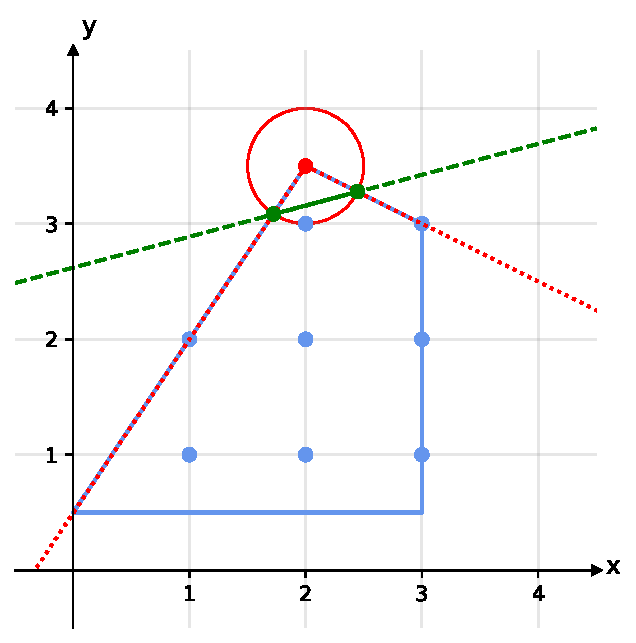
\includegraphics[width=0.5\textwidth]{Images/intersection_cut.pdf}
    \caption{Diagram of intersection cut for \cref{problem:mip_example}}
    \label{fig:intersection_cut}
    \subcaption*{
        The feasible points of the MIP are the integer points respecting the polyhedral constraints (blue points). The set of feasible solutions to the relaxed LP are all the points in the interior or on the boundary of the polytope (blue line segments). The optimal solution $\bold{ \tilde x}$ to the relaxed LP is the point in the feasible region with the biggest $y$-value (red point). A possible $S$-free set $C$ is a disk with center $\bold{\tilde x}$ and the radius being the distance between $\bold{\tilde x}$ and the closest integer (red circle). The conic relaxation are the extreme rays generated by $\bold{\tilde x}$ which correspond to the two active constraints at $\bold{\tilde x}$ (is indicated by the dotted, red line). The intersection of the conic relaxation and $C$ are the two points in green. The intersection cut is constructed with the line going through the intersecting points (dashed line in green). The area above the green line will be cut off and $\bold{\tilde x}$ is no longer a feasible solution.}
\end{figure} 

The conic relaxation at $\bold{\tilde x}$ is a pointed cone with extreme point $\bold{\tilde x}$ and can be written as: 
\begin{equation} \label{Eq:conic_relaxation}
    P' = \{ \bold{\tilde x} + \sum_{j=1}^n \lambda_j \mathbf r^j : \boldsymbol \lambda \geq 0 \}
\end{equation}
or as:
\begin{equation} \label{Eq:conic_relaxation_polyhedral}
    P' = \{\mathbf x|\bold{\tilde Ax} \leq \bold{\tilde b}\}
\end{equation} 
%\unsure[inline]{confusing to have two x?}
where $\mathbf r^j$ are the extreme rays, $\bold{\tilde A}$ is an invertible $n\times n$ submatrix of $ \mathbf A$ such that the rows are linearly independent and are a basis for $\bold{\tilde x}$ \cite{bienstock_outer_product_free_sets}. 
% If the original problem is brought in the form $ \mathbf Ax \leq b$, the bounds on $x$ are included in $ \mathbf A$ and therefore $m \geq n$. 
A basis for $\bold{\tilde x}$ are the nonbasic constraints at $\bold{\tilde x}$.
\enlargethispage{\baselineskip}
If a constraint is nonbasic, the corresponding slack variable of the standard form is nonbasic and therefore 0. 
This implies that the constraint is active. 

\newpage
Going back to \cref{problem:mip_example}, the polyhedral presentation of the conic relaxation at $(2, 3.5)$ is:
\begin{equation*}
    P' =     
    \left\{ (x,y) \Bigg|
        \left[ \begin{array}{cc}
            -1.5 & 1 \\
            0.5 & 1
        \end{array}\right]
        \left[ \begin{array}{c}
            x \\ y
        \end{array} \right] \leq
        \left[ \begin{array}{c}
            0.5 \\ 4.5
        \end{array} \right] 
    \right\}
\end{equation*}

The inverse of $\bold{\tilde A}$ is 
\begin{equation*}
    \bold{\tilde A}^{-1} =     
        \left[ \begin{array}{cc}
            -0.5 & 0.5 \\
            0.25 & 0.75
        \end{array}\right]
\end{equation*}
and we get the extreme rays $r_1 = (0.5 -2.5)$ and $r_2= (-0.5, -0.75)$.

After deriving the conic relaxation, we have $\bold{\tilde x} = \bold{\tilde A}^{-1} \bold{\tilde b}$ and $\mathbf r^j= - \bold{\tilde A}^{-1}_{*,j}$ \cite{bienstock_outer_product_free_sets}. For each extreme ray $\mathbf r^j$ there either exists an intersection with the boundary of $C$ in which case $\lambda^*_j > 0$ is the step length or the extreme ray is contained in $C$ and $\lambda^*_j= \infty$.
The \textit{intersection cut} is defined as \cite{bienstock_outer_product_free_sets}:
\begin{equation} \label{Eq:interscetion_cut}
    \sum_{i=1}^n (\bold{\tilde a}_{i,*} \mathbf x - \tilde b_i)/ \lambda_i^* \leq -1
\end{equation}
 where $\bold{\tilde a}_{i,*}$ denotes the $i$-th row of basic constraints $\bold{\tilde A}$.\\
% \unsure[inline]{do we need transpose here? \\MB: depends how you define your notation. It would make more sense to define the selected column as a column vector and use the transpose \\ matches outer-product-free set paper}
\unsure[inline]{remove equation? or move to appendix?}
If we reformulate \cref{Eq:interscetion_cut}, we see that it matches the definition of a cut in \cref{Eq:cuts} \cite{bienstock_outer_product_free_sets}:
\begin{align}
    \sum_{i=1}^n (\bold{\tilde a}_{i,*} \mathbf x - \tilde b_i)/ \lambda_i^* &\leq -1 \\
    \sum_{i=1}^n ((1/ \lambda_i^*) \bold{\tilde a}_{i,*} \mathbf x - (1/ \lambda_i^*)\tilde b_i) &\leq -1 \\ 
    \sum_{i=1}^n (1/ \lambda_i^*) \bold{\tilde a}_{i,*} \mathbf x - \sum_{i=1}^n  (1/ \lambda_i^*)\tilde b_i &\leq -1 \\
    \sum_{i=1}^n (1/ \lambda_i^*) \bold{\tilde a}_{i,*} \mathbf x & \leq -1 + \sum_{i=1}^n  (1/ \lambda_i^*)\tilde b_i
\end{align}
\begin{equation*}
    \alpha_0 = -1 + \sum_{i=1}^n  (1/ \lambda_i^*)\tilde b_i \quad \quad \alpha_j = \sum_{i=1}^n (1/ \lambda_i^*) \bold{\tilde a}_{i,j} \mathbf x
\end{equation*}

% \todo[inline]{explain why x is cut off}
\todo[inline]{update: basis defining x and basis for P}

% \unsure[inline]{does opt sense matter?\\MB: no it doesn't, intersection cuts don't cut off the objective}
% \todo[inline]{different cut formulations}
% \todo[inline]{use bar or tilde in intersection cuts? tilde already used for combinatorial benders}
